\chapter{Wybrane zagadnienia analizy semantycznej języka naturalnego}

Analiza semantyczna jest trudnym zagadnieniem ze względu na złożoność języków naturalnych. Często ich reguły są skomplikowane, zawierają znacznie więcej wyjątków niż języki formalne, które są prostsze w przetwarzaniu komputerowym. Znaczenie poszczególnych wyrazów może być zależne od kontekstu całego zdania bądź akapitu.

\section{Przetwarzanie języka naturalnego}

\subsection{Word Embeddings}
Word Embeddings to jedna z technik przetwarzania języka naturalnego  (ang. \textit{Natural Language Processing, NLP}) służąca do modelowania języka i ekstrahowania informacji z zapisu tekstowego. W dużym uproszeniu, Word Embedding polega na reprezentowaniu znaczeń słów lub zdań jako wielowymiarowe wektory abstrakcyjnych numerycznych cech. Motywacją przemawiającą za wykorzystaniem takiej reprezentacji danych jest fakt, iż komputery nie radzą sobie z analizowaniem tekstu w postaci ciągu znaków. Wartości numeryczne są naturalnym formatem danych wejściowych w większości systemów realizujących algorytmy przetwarzania danych. Metody tworzenia takich powiązań oparte są na statystyce, macierzach współwystąpień (\textit{ang. co-occurence matrix}) i sieciach neuronowych.

\subsubsection{Wektor wystąpień (\textit{ang. Count Vector})}
Rozważmy korpus $C$ składający się z $D$ dokumentów $\{d_1, d_2,..., d_D\}$ i N unikatowych wyrazów wydobytych z korpusu $C$. Niech to $N$ wyrazów jest naszym słownikiem, a rozmiar macierzy wektorów wystąpień to $D \times N$. Każdy wiersz macierzy zawiera częstotliwość wystąpienia wyrazów w dokumencie $d(i)$, gdzie $i = \{1, 2, ... ,D\}$.

\subsubsection{Macierz współwystąpień}
Reprezentacja danych polegająca na zliczeniu wystąpień słów $w1$ i $w2$ w obszarze okna o stałym rozmiarze. Rozważmy korpus $C$ składający się z $N$ unikalnych słów. Macierz wpółwystąpień będzie miała rozmiar $N \times N$. Zaletą macierzy współwystąpień jest zachowanie relacji między słowami, niestety wadą takiej reprezentacji danych jest duże zapotrzebowanie pamięci przy przetwarzaniu większej ilości tekstu.

\subsubsection{CBOW}
CBOW to algorytm tworzący Word Embeddingi z wykorzystaniem sieci neuronowej. CBOW próbuje przewidzieć wystąpienie słowa w kontekście innych słów. Architekura sieci wykorzystanej w algorytmie CBOW składa się z 3 warstw:
\begin{itemize}
  \item Warstwa wejściowa to macierz o rozmiarze $X \times V$ gdzie każdy wiersz to wektor zer i jedynek, w którym wartość 1 oznacza wystąpienie danego słowa w zadanym kontekście. $V$ to liczba unikatowych słów w korpusie,
  \item Warstwa ukryta zbudowana z $N$ neuronów o liniowej funkcji aktywacji,
  \item Warstwa wyjściowa będąca $V$-wymiarowym wektorem prawdopodobieństw wystąpienia słowa w danym kontekście.
\end{itemize}
Aktywacja warstwy ukrytej jest traktowana jako wektorowa reprezentacja zadanego słowa.
Architektura to została zilustrowana na rysunku~\ref{fig:cbow}.
\begin{figure}[H]
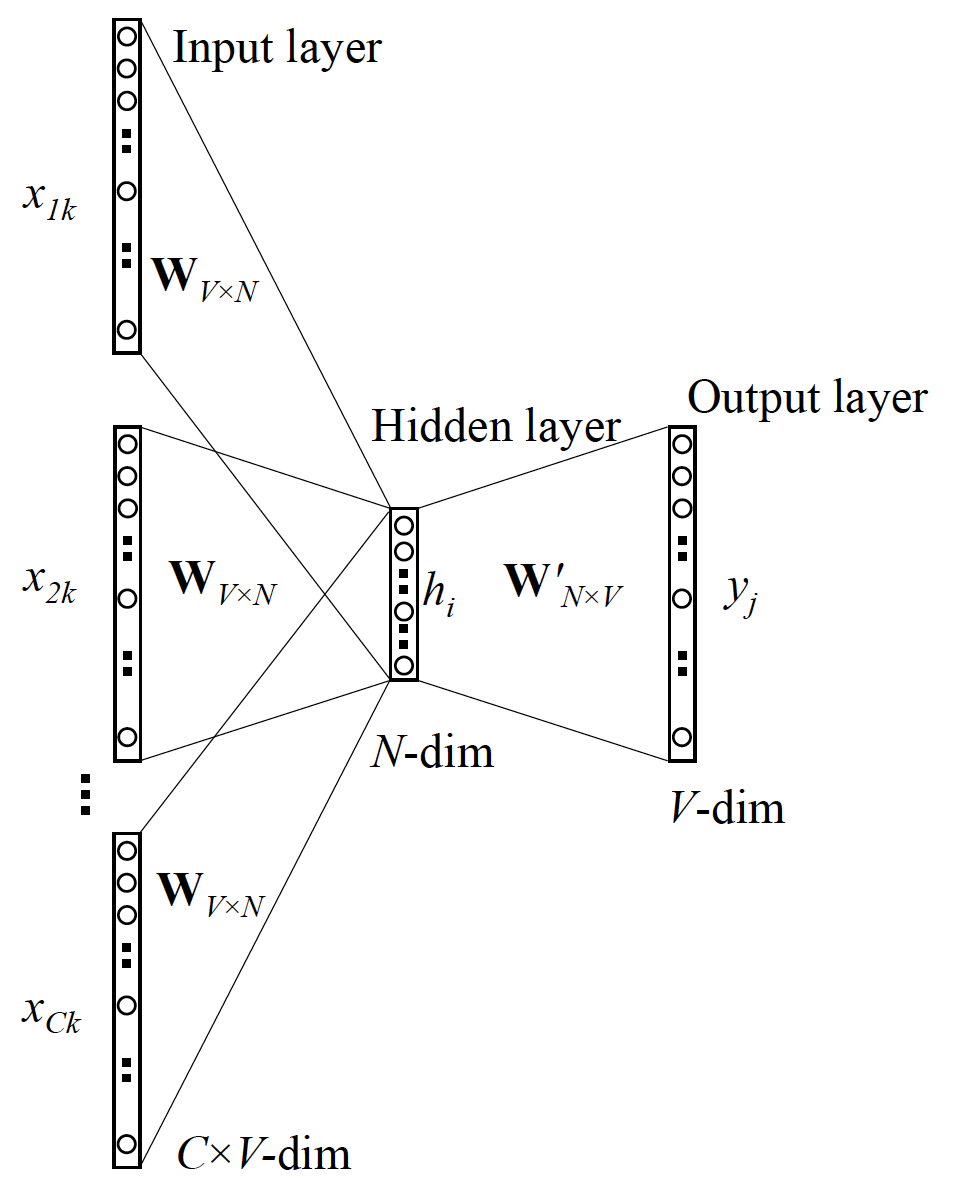
\includegraphics[scale=0.2]{fig-word2vec-cbow}
\centering
\caption{Architekura sieci wykorzystanej w algorytmie CBOW. %AL%%%- źródło?
\label{fig:cbow}}
\end{figure}

\subsection{Miary podobieństwa}

\subsubsection{Indeks Jaccarda}
Indeks Jaccarda to miara oparta na algebrze zbiorów. Wyraża się ją wzorem:
%\[
\begin{equation}
  J(A,B) = \frac{|A \bigcap B|}{|A \bigcup B|}
\end{equation}
%\]

Gdzie:
\begin{itemize}
\item A, B - skończone zbiory
\item $J(A,B)$ - wartość indeksu Jaccarda
\end{itemize}
Wartość indeksu zawiera się w zbiorze $\langle 0,1 \rangle$. Jeżeli oba zbiory są puste, jako wartość indeksu przyjmuje się 1. W przypadku przetwarzania języka, można zastosować tą miarę do wyrażenia podobieństwa dwóch tekstów. Tekst należy w tym celu przedstawić jako zbiór tokenów, czyli rdzeni słów. Dla tak utworzonych zbiorów można zastosować indeks Jaccarda.
Prostota, choć jest niewątpliwą zaletą tej miary, rodzi również pewne problemy. Po pierwsze, reprezentacja w postaci zbioru nie pozwala odzwierciedlić informacji jaką może nieść kolejność słów. Po drugie, nie są uwzględniane synonimy, a zatem dwa teksty o podobnym znaczeniu, ale złożone z różnych wyrazów otrzymają niską wartość podobieństwa.

\subsubsection{Podobieństwo kosinusowe}
Wygodną miarą podobieństwa dla tekstu reprezentowanego w postaci wektorów może być podobieństwo kosinusowe, czyli wartość funkcji kosinus. Taka miara może być użyta dla wektorów o dowolnej liczbie wymiarów. Dodatkowo, dla wektorów z dodatniej przestrzeni będzie przyjmowała wartości z przedziału $\langle 0,1 \rangle$.
Podobnie jak indeks Jaccarda, podobieństwo kosinusowe charakteryzuje prostota. Jednak w tym przypadku, miara operuje na bardziej trafnej reprezentacji tekstu i nie powoduje utraty informacji.

\subsubsection{Długość tekstu}
Inną, prostą metodą określania podobieństwa tekstów może być porównanie długości. Miara, choć naiwna, może niekiedy być użyteczna. Można podejrzewać, że dwa teksty o podobnym znaczeniu będą miały zbliżoną długość, natomiast duże różnice w długości mogą oznaczać znaczną rozbieżność treści. 
W praktyce miara długości okazuje się jednak mało trafna i nie daje zadowalających wyników. 



